\section{Block Diagram}

To verify the model in simulation \eqref{FrameEq4TaylerApprox} is transformed into the Laplace domain, after which a transfer function of the system is derived. The proceeding equations are valid only around the operating point, and so for better overview, in the following \si{\Delta \theta_F = \theta_F}.
%
\begin{flalign}
	\eq{(J_F+m_w \cdot {l_w}^{2}) \cdot \theta_F \cdot s^2}{-B_F \theta_F\cdot s +  ( m_F \cdot l_F + m_w \cdot l_w ) g \cdot \theta_F - \tau_m + B_w \theta_w\cdot s } & \nonumber\\
\label{LaplaceOfLinearizedModel}
\end{flalign}
%
The angle of the reaction wheel, \si{\theta_w}, still features in \eqref{LaplaceOfLinearizedModel}. It is desirable to have only one input, \si{\tau_m}, and one output, \si{\theta_F}. To achieve this, \eqref{WheelRotEq2} is transformed into the Laplace domain and solved for \si{\theta_w}.
%
\begin{flalign}
	\eq{\theta_w\cdot s^2} {\frac{\tau_m - B_w \theta_w\cdot s}{J_w} - \theta_F\cdot s^2}   &\\
	\eq{\theta_w} {\frac{ -J_w \theta_F \cdot s^2 + \tau_m }{ J_w \cdot s^2 + B_w \cdot s }}&
\label{WheelRotEq2Laplace}
\end{flalign}
%
\Eqref{WheelRotEq2Laplace} is now substituted for \si{\theta_w} in \eqref{LaplaceOfLinearizedModel}, and the transfer function is of the system is derived.
%
\begin{flalign}
	\eqOne{(J_F+m_w \cdot {l_w}^{2}) \cdot \theta_F \cdot s^2}{-B_F \theta_F\cdot s +  ( m_F \cdot l_F + m_w \cdot l_w ) \cdot g \cdot \theta_F - \tau_m}
	\eqTwo{+ B_w \cdot \left( \frac{ -J_w \theta_F \cdot s^2 + \tau_m }{ J_w \cdot s^2 + B_w \cdot s} \right)\cdot s }&\nonumber
\label{CubliTransferFunction}
\end{flalign}

\vspace{-.2cm}
\large{\si{\frac{\theta_F}{\tau_m} =}}\nolinebreak
\Large{
\si{\frac{\frac{s}{-J_F - m_w \cdot {l_w}^2}}{s^3 + \left( \frac{B_w}{J_w} + \frac{B_w + B_F}{J_F + m_w \cdot {l_w}^2} \right) s^2 - \left( \frac{ \left( m_F \cdot l_F + m_w \cdot l_w \right)\cdot g}{ \left( J_F + m_w \cdot {l_w}^2 \right) J_w} - \frac{B_F B_w}{ \left(J_F + m_w \cdot {l_w}^2 \right) J_w} \right) s - \frac{\left(m_F \cdot l_F + m_w \cdot l_w \right) B_w\cdot g}{\left(J_F + m_w \cdot {l_w}^2 \right) J_w} }}}\normalsize\vspace{-1.9cm}\\
\vspace{1.8cm}\begin{flalign}\label{2ndCubliTransferFunction}\end{flalign}
%
The transfer function from \eqref{2ndCubliTransferFunction} can also be represented in the form of a block diagram, as seen in \figref{cubliSimulink}.

% \begin{figure}[H] 
% 	\centering 
% 	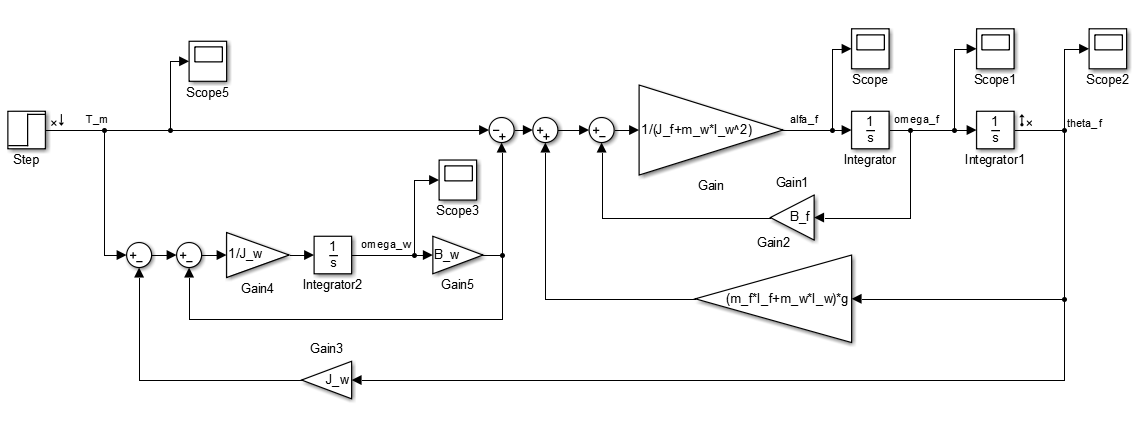
\includegraphics[scale=0.53]{figures/cubliSimulink}
% \end{figure}
% \end{figure} 
\begin{figure}[H]
	  \begin{tikzpicture}[ auto,
                       thick,                         %<--setting line style
                       node distance=1.5cm,             %<--setting default node distance
                       scale=0.75,                     %<--|these two scale the whole thing
                       every node/.style={scale=0.62}, %<  |(always change both)
                       >=triangle 45 ]

    %-- Blocks creation --%
    \draw
      % DIRECT TERM %
      node[shape=coordinate][](input1) at (0,0){}
      node[shape=coordinate][](feedForward) at (0.5,0){}
      node(sum1) at (7.75,0) [sum] {$\sum$}
      node(sum2) at (9.25,0) [sum]{$\sum$}
      node(sum3) at (10.75,0) [sum]{$\sum$}

      node(torque2rotacc1) at (12.85,0) [block]{\Large $\frac{1}{J_F + m_w \cdot {l_w}^{2}}$}

      node(integration1) at (15.75,0) [block] {\Large $\frac{1}{s}$}
      node(integration2) at (18.2,0) [block] {\Large $\frac{1}{s}$}

      node[shape=coordinate][](output) at (19,0){}
      node[shape=coordinate][](veloFeedbackNode) at (16.8,0){}
      node[shape=coordinate][](accFeedbackNode) at (14.5,0){}
    ;
    \draw
      % REACTION WHEEL EQUATIONS %  
      node(sum4) at (1.5,-2) [sum]{$\sum$}
      node(sum5) at (2.85,-2) [sum]{$\sum$}

      node(torque2rotacc2) at (4.3,-2) [block]{\Large $\frac{1}{J_w \cdot s}$}
      % node(integration3) [block, right of = torque2rotacc2] {$\frac{1}{s}$}
      node(frictionWheel) at (6.9,-2) [block] {\Large $B_w$}

      node[shape=coordinate][](veloWheelFeedback) at (7.75,-3.5){}
    ;
    \draw
      % FEEDBACKS %
      node(accFeedback) at (4, -6) [block] {\Large $J_w$}
      node(veloFeedback) at (12.65,-2) [block] {\Large $B_F$}
      node(angleFeedback) at (11.65,-4) [block] {\Large $(m_F \cdot l_F + m_w \cdot l_w)g$}
    ;
    %-- Block linking --%
    % INPUT %
    \draw[-](input1)        -- node{\Large $\tau_m(s)$}(feedForward);
    \draw[->](feedForward)  -- (sum1);

    % OUTPUT %
    \draw[-](integration2)  -- (output);
    \draw[->](output)       -- node {\Large $\theta_{F}(s)$} (20,0);

    % DIRECT TERM %
    \draw[->] (sum1)            -- (sum2);
    \draw[->] (sum2)            -- (sum3);
    \draw[->] (sum3)            -- (torque2rotacc1);
    \draw[->] (torque2rotacc1)  -- node{\Large $\alpha_F(s)$}(integration1);
    \draw[->] (integration1)    -- node{\Large $\omega_F(s)$}(integration2);

    % REACTION WHEEL EQUATIONS %
    \draw[->] (feedForward)     |- (sum4);
    \draw[->] (sum4)            -- (sum5);
    \draw[->] (sum5)            -- (torque2rotacc2);
    \draw[->] (torque2rotacc2)  -- node{\Large $\omega_w(s)$}(frictionWheel);
    % \draw[->] (integration3)    -- (frictionWheel);
    \draw[->] (frictionWheel)   -| (sum1);

    \draw[-] (frictionWheel)       -| (veloWheelFeedback);
    \draw[->] (veloWheelFeedback)  -| (sum5);

    % FEEDBACKS
    \draw[->] (accFeedbackNode)  |- (accFeedback);
    \draw[->] (accFeedback)      -| (sum4);

    \draw[->] (output)           |- (angleFeedback);
    \draw[->] (angleFeedback)    -| (sum2);

    \draw[->] (veloFeedbackNode) |- (veloFeedback);
    \draw[->] (veloFeedback)     -| (sum3);

    %-- Nodes --%
    \draw%--------------------------------------------------------------
      node at (input1)            [shift={(-0.04, -0.05 )}] {\Large \textopenbullet}
      node at (output)            [shift={( 0.007, -0.05 )}] {\Large \textbullet}
      node at (veloFeedbackNode)  [shift={( 0.007, -0.05 )}] {\Large \textbullet}
      node at (accFeedbackNode)   [shift={( 0.007, -0.05 )}] {\Large \textbullet}
      node at (feedForward)       [shift={( 0.007, -0.05 )}] {\Large \textbullet}
      node at (frictionWheel)     [shift={( 1.025, -0.04 )}] {\Large \textbullet}
    ;

    %-- Summation signs --%
      \draw%--------------------------------------------------------------
      node at (sum1) [right = -6.6mm, below = .6mm] {$-$}
      node at (sum1) [right = -3mm, below = 3.9mm]  {$+$} 
      node at (sum2) [right = -6.6mm, below = .6mm] {$+$}
      node at (sum2) [right = -3mm, below = 3.9mm]  {$+$}
      node at (sum3) [right = -6.6mm, below = .6mm] {$+$}
      node at (sum3) [right = -3mm, below = 3.9mm]  {$-$}
      node at (sum4) [right = -6.6mm, below = .6mm] {$+$}
      node at (sum4) [right = -3mm, below = 3.9mm]  {$-$}
      node at (sum5) [right = -6.6mm, below = .6mm] {$+$}
      node at (sum5) [right = -3mm, below = 3.9mm]  {$-$}
    ;

  \end{tikzpicture}
	\caption{Block diagram of the Cubli system. The reference is the desired torque that the wheel acts on the frame with. Output is the angle of the Cubli frame}
	\label{cubliSimulink}
\end{figure}

